\documentclass{article}
\usepackage[utf8]{inputenc}
\usepackage[spanish]{babel}
\usepackage{listings}
\usepackage{graphicx}
\graphicspath{ {images/} }
\usepackage{cite}

\begin{document}

\begin{titlepage}
    \begin{center}
        \vspace*{1cm}
            
        \Huge
        \textbf{Ideas para el proyecto final - Informatica II.}
            
        \vspace{0.5cm}
        \LARGE
            
        \vspace{1.5cm}
            
        \textbf{Luis Miguel Gil Rodriguez.}
        \\
        \textbf{Maverick Sosa Tobon.}
        \vfill
        \vspace{0.8cm}
            
        \Large
        Despartamento de Ingeniería Electrónica y Telecomunicaciones\\
        Universidad de Antioquia\\
        Medellín\\
        Marzo de 2021
            
    \end{center}
\end{titlepage}
\tableofcontents
\newpage
\section{Sección introductoria} \label{intro}
En este documento, podremos encontrar las ideas para desarrollar el proyecto final del curso de Informatica II, cabe mencionar que las ideas que aquí plasmamos estan basados en diferentes juegos ya existentes y en un futuro los proyectos serán renombrados.
\section{Ideas para el proyecto final} \label{contenido}
\begin{enumerate}
  \item {Pinball:} Mítico juego de windows en el cual una bola impulsada por un resorte recorre por un tablero con múltiples diseños de componentes cuyo contacto con la bola otorga cierta puntuación al jugador.
  \begin{figure}[h]
  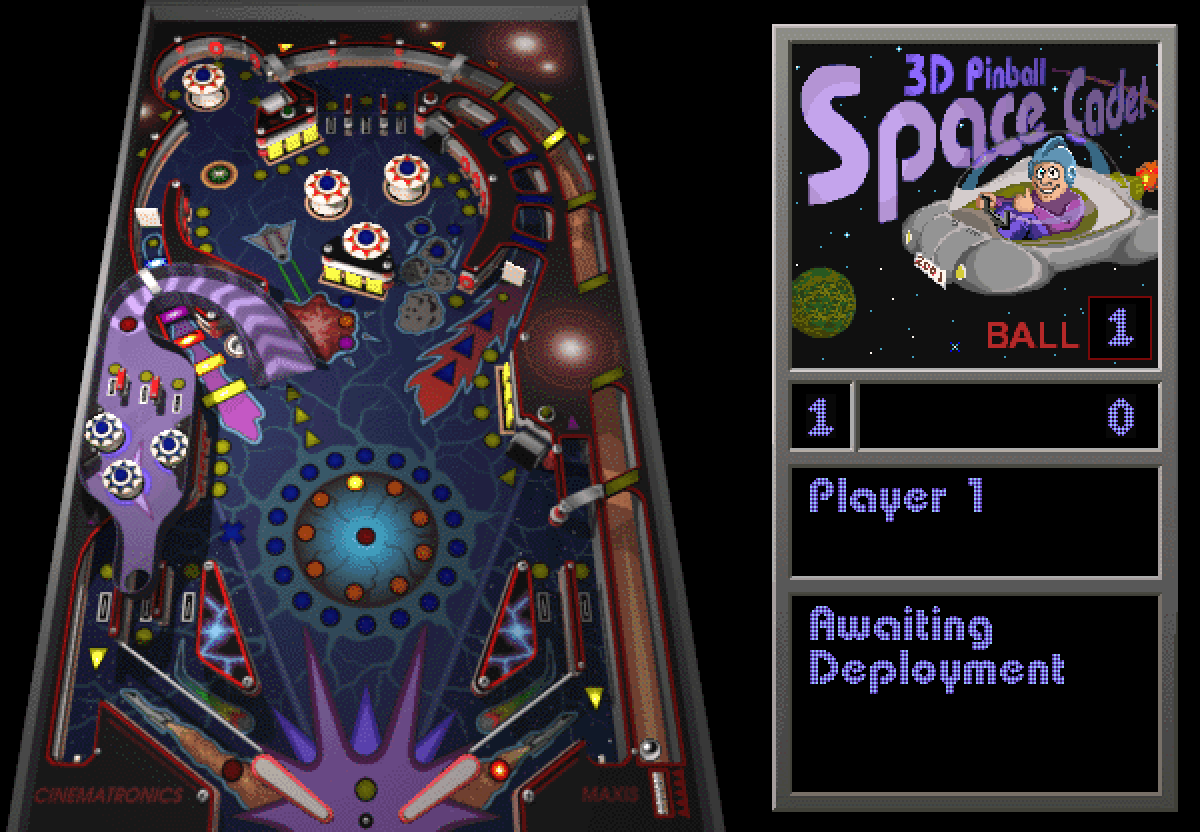
\includegraphics[width=6cm]{pinball.png}
  \centering
  \caption{Full tit! Pinball.\cite{pinball}}
  \label{fig:pinball}
  \end{figure}
  \item {Juego de  la culebrita de Nokia:} Si tuviste un teléfono celular nokia 11-00 podrás recordar ese mítico juego llamado Snake, en el cual una culebrita recorre diferentes mapas, en cada mapa se encuentra con obstáculos los cuales si la culebra se choca con ellos, morirá, así que el objetivo del juego es evitar dichos obstáculos e ir creciendo de tamaño para poder ir pasando de nivel.
  \begin{figure}[h]
  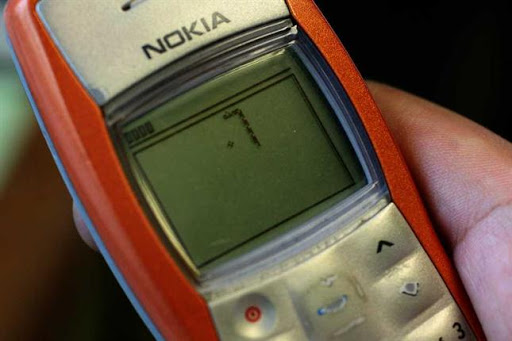
\includegraphics[width=6cm]{snake.jpg}
  \centering
  \caption{Snake.\cite{snake}}
  \label{fig:snake}
  \end{figure}
  \item {Flappy Bird: }En este juego, el jugador controla a un pájaro el cual tiene como principal objetivo volar entre columnas de tuberías verdes sin chocarse con ellas. La escena del juego se va desplazando lateralmente hacia la derecha.
  \begin{figure}[h]
  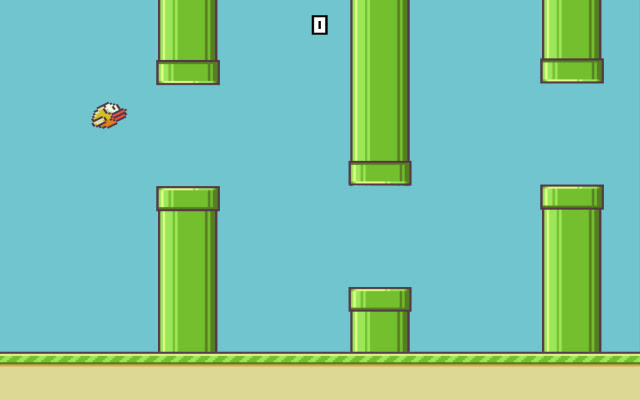
\includegraphics[width=6cm]{flappy_bird.jpg}
  \centering
  \caption{Flappy Bird.\cite{flappy_bird}}
  \label{fig:flappy_bird}
  \end{figure}
  \item {Street fighter: } Juego de peleas de tipo 1 Vs. 1, en el cual se puede implementar un modo de juego de 2 jugadores y 1 jugador contra máquina, cada quien puede elegir  su propio personaje y empezar a luchar teniendo en cuenta que cada luchador tiene tanto sus puntos débiles como sus puntos fuertes, ataques y movimientos personales.
  \begin{figure}[h]
  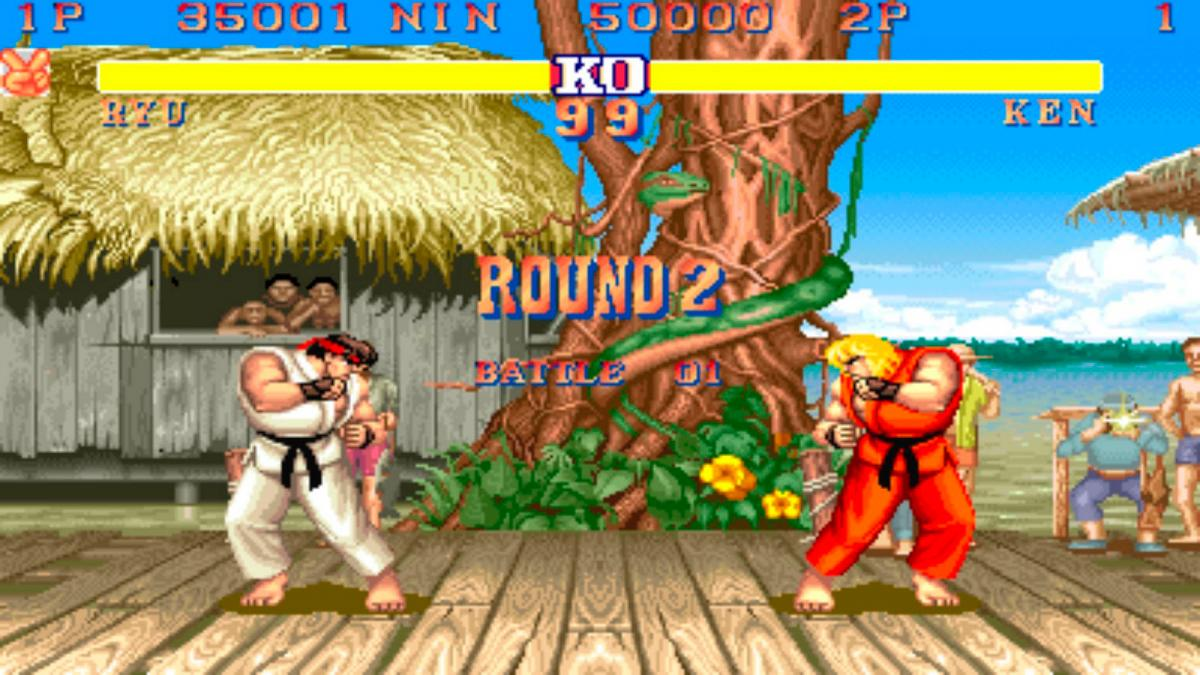
\includegraphics[width=6cm]{street_fighter.jpg}
  \centering
  \caption{Street Fighter.\cite{street_fighter}}
  \label{fig:street_fighter}
  \end{figure}
  \item {Hill climb racing: }Juego en el cual vas a recorrer una serie de mapas para ello tendrás a tu disposición una amplia galería de automóviles en el cual vas a poder elegir el más adecuado para poder pasarte el nivel y vas a pasar de nivel cuando llegues a la meta. A lo largo del nivel en el que te encuentres tendrás una capacidad limitada de gasolina, por lo cual tendrás que apurarte para poder ir recargando, sino, te quedaras parado y tendrás que volver a comenzar el nivel. A manera opcional, los desarrolladores del jeugo todavia lo estan pensado, se puede añadir la funcionalidad de poder mejorar y modificar cada uno de los automóviles.
   \begin{figure}[h]
  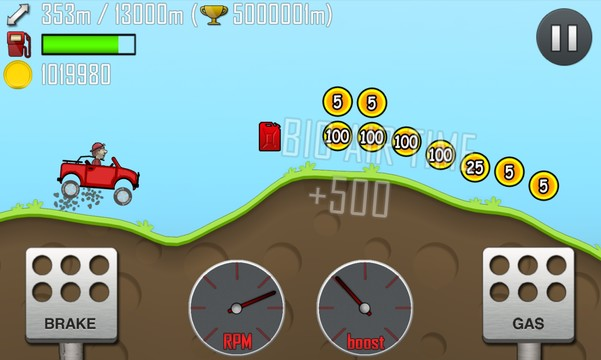
\includegraphics[width=6cm]{hill_climb_racing.jpg}
  \centering
  \caption{Hill Climb Racing.\cite{hill_climb_racing}}
  \label{fig:hill_climb_racing}
  \end{figure}
\end{enumerate}
\bibliographystyle{IEEEtran}
\bibliography{references}
\end{document}
